% floats.tmpl.tex: figure and table environments of the main text, one block per float, introduced by a marker line
% "%%FLOAT <label>". src/paper/build_paper.py fills this file (fill_ledger), splits it at the markers and places each float
% after the paragraph that holds its first \ref (paper/LABELS.md; SPEC s3; research/FIGURES_PLAN.md; paper/FIGURE_CHANGES.md).
% Widths: \FigD = double column (190 mm in print), \FigM = 1.5 column (140 mm), \FigS = single column (90 mm); defined in main.tmpl.tex.
% Captions: finding, n, interval type, "stress test" where injected quantities are shown. Numbers are placeholders only.
% Table numbers follow the order of placement: methods, data, accuracy, confirmatory, secondary.

%%FLOAT fig:design
\begin{figure}[tp]
\centering
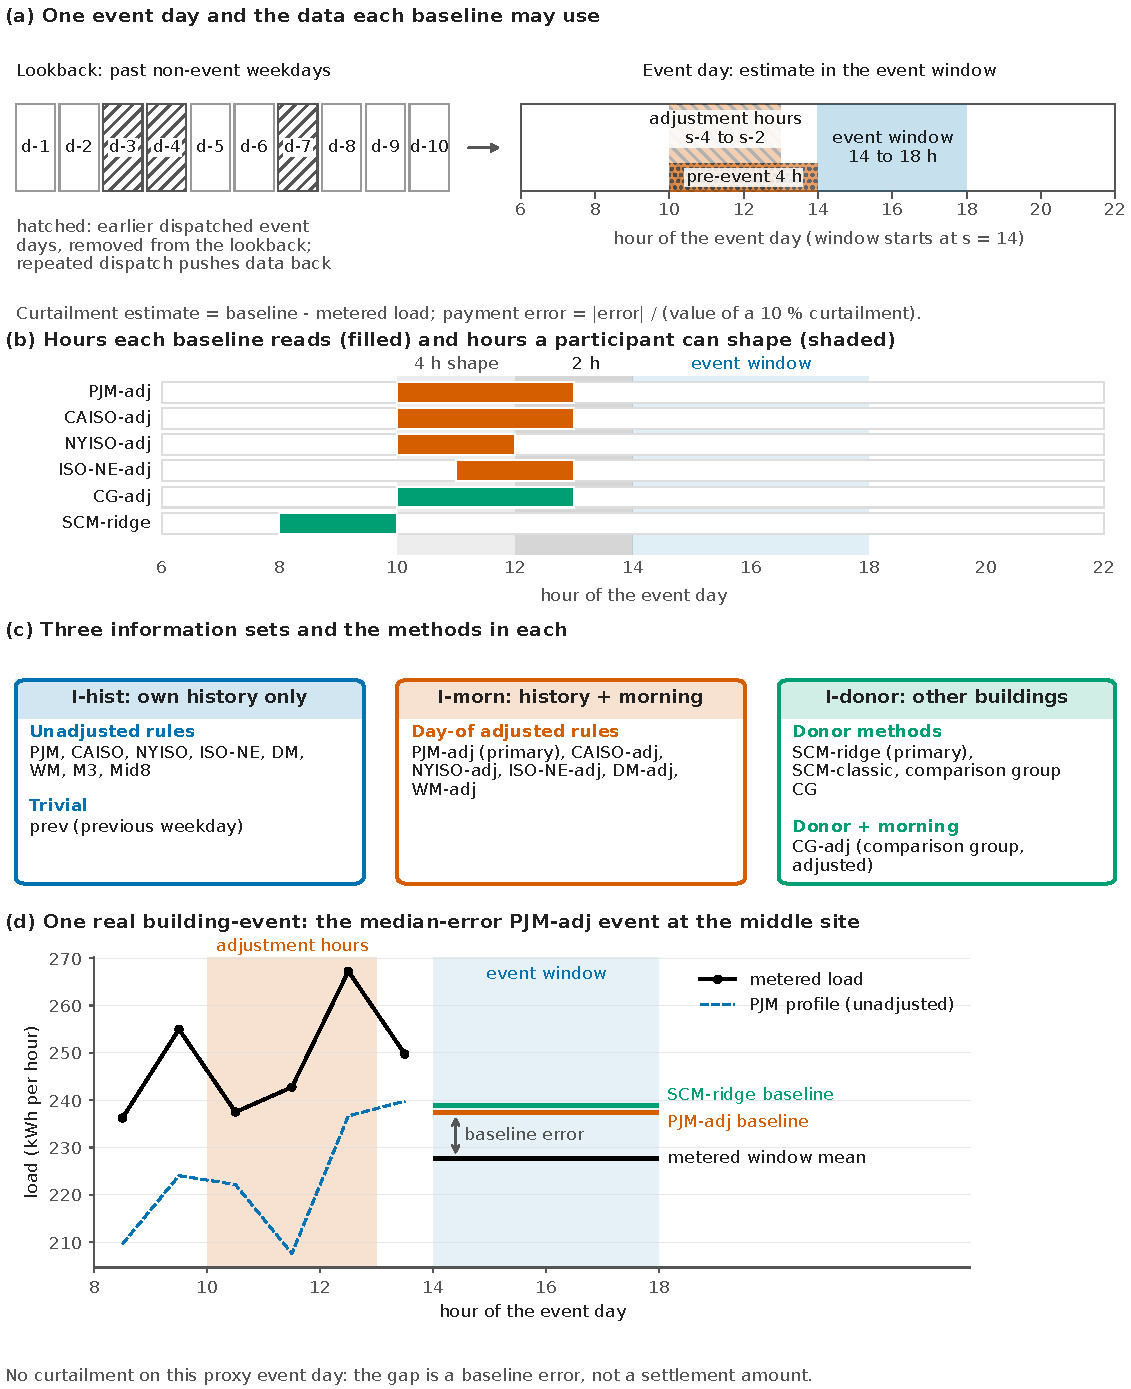
\includegraphics[width=\FigOne]{figures/fig_01_design.pdf}
\caption{Design of the study: the hours each baseline reads and the hours a participant can shape. (a) Lookback days, with dispatched days removed under repeated dispatch. (b) Hours read versus hours shaped for six baselines. (c) Information sets. (d) One real building-event with its baselines and settlement gap (plot only). Day-of adjustment reads the hours before the window, SCM-ridge reads none of the four-hour shaped hours, and no method reads the target's own load inside the window.}\label{fig:design}
\end{figure}

%%FLOAT tab:methods
\begin{table}[tp]
\centering
\caption{Compact list of baseline methods by information set, with definition, lookback, adjustment and cap. The full list with sources is Supplement Table~\ref{tabS:methodsfull}.}\label{tab:methods}
\scriptsize
\setlength{\tabcolsep}{2.5pt}
\begin{tabular}{>{\raggedright\arraybackslash}p{1.9cm}>{\raggedright\arraybackslash}p{1.7cm}>{\raggedright\arraybackslash}p{4.4cm}>{\raggedright\arraybackslash}p{2.2cm}>{\raggedright\arraybackslash}p{3.2cm}>{\raggedright\arraybackslash}p{1.9cm}}
\toprule
Method & Information set & Definition & Lookback & Adjustment & Cap \\
\midrule
prev & I-hist & Previous eligible weekday & 1 day & none & none \\
PJM & I-hist & PJM weekday baseline (highest 4 of 5 recent weekdays) & 45 days & none & none \\
PJM-adj & I-morn & PJM with day-of adjustment (primary rule) & 45 days & additive, hours s$-$4..s$-$2 & none \\
CAISO & I-hist & CAISO 10-in-10 & 45 days & none & none \\
CAISO-adj & I-morn & CAISO 10-in-10 with adjustment & 45 days & ratio, hours s$-$4..s$-$2 & [0.8, 1.2] \\
NYISO-adj & I-morn & NYISO with adjustment & 30 days & ratio, hours s$-$4, s$-$3 & [0.8, 1.2] \\
ISO-NE-adj & I-morn & ISO-NE with adjustment & 30 days & additive, hours s$-$3, s$-$2 & floor 0 \\
WM-adj & I-morn & Weather matching with adjustment & 90 days & ratio, hours s$-$4, s$-$3 & [0.6, 1.4] \\
CG & I-donor & Comparison group, unadjusted PJM ratio & 45 days + donors & none & none \\
CG-adj & I-donor + I-morn & Comparison group, PJM-adj ratio & 45 days + donors & additive, hours s$-$4..s$-$2 & none \\
SCM-ridge & I-donor & Ridge synthetic control (primary donor method) & 7 weekdays + morning & donor weights & weights sum to one \\
\bottomrule
\end{tabular}
\par\smallskip{\footnotesize\raggedright Hours $s-4,\dots$ are relative to the window start $s$. All other evaluated methods, the sources, document vintages and the methods without results are in Supplement Table~\ref{tabS:methodsfull}. CAISO and ISO-NE unadjusted baselines coincide (Table~\ref{tab:accuracy}).\par}

\end{table}

%%FLOAT fig:sample
\begin{figure}[tp]
\centering
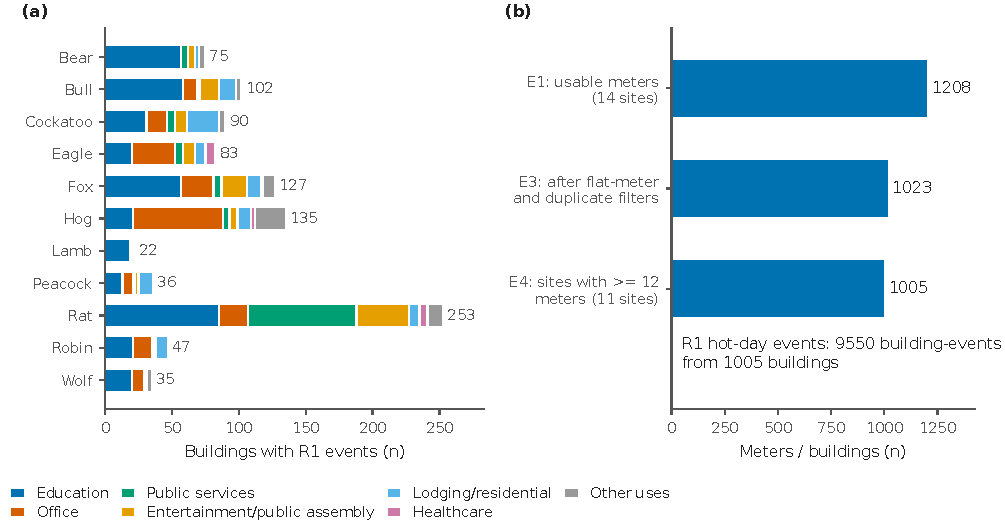
\includegraphics[width=\FigD]{figures/fig_02_sample.pdf}
\caption{Sample of 1{,}005 buildings at 11 campus-heavy sites. (a) Buildings by site and primary use. (b) Eligibility funnel from valid meters to hot-day building-events (R1).}\label{fig:sample}
\end{figure}

%%FLOAT tab:accuracy
\begin{table}[tp]
\centering
\caption{Hot-day (R1) and random-weekday (R3) accuracy by method: building-pooled medians of relMAE, signed bias ($e=B-L$; positive means over-payment) and payment error ratio (PER), with order-statistic 95\,\% intervals of the site medians. LightGBM rows give the fixed-parameter and the tuned (pre-registered 40-trial search on 2016) variants; MLP rows are tuned variants only.}\label{tab:accuracy}
\scriptsize
\setlength{\tabcolsep}{2.5pt}
\begin{tabular}{>{\raggedright\arraybackslash}p{3.0cm}>{\raggedright\arraybackslash}p{1.5cm}>{\raggedleft\arraybackslash}p{1.0cm}>{\raggedleft\arraybackslash}p{1.0cm}>{\raggedleft\arraybackslash}p{1.0cm}>{\raggedleft\arraybackslash}p{1.0cm}>{\raggedleft\arraybackslash}p{1.0cm}>{\raggedleft\arraybackslash}p{1.0cm}>{\raggedleft\arraybackslash}p{2.1cm}>{\raggedleft\arraybackslash}p{2.1cm}}
\toprule
Method & Information set & R1 relMAE & R1 bias & R1 PER & R3 relMAE & R3 bias & R3 PER & R1 relMAE interval & R1 bias interval \\
\midrule
prev & I-hist & 0.079 & $-$0.037 & 0.79 & 0.075 & 0.009 & 0.75 & [0.057, 0.109] & [$-$0.068, 0.004] \\
PJM & I-hist & 0.083 & $-$0.024 & 0.83 & 0.088 & 0.037 & 0.88 & [0.059, 0.130] & [$-$0.067, 0.071] \\
PJM-adj & I-morn & 0.047 & 0.000 & 0.47 & 0.054 & 0.007 & 0.54 & [0.042, 0.064] & [$-$0.009, 0.017] \\
CAISO / ISO-NE (identical) & I-hist & 0.094 & $-$0.039 & 0.94 & 0.094 & 0.017 & 0.94 & [0.060, 0.118] & [$-$0.083, 0.013] \\
CAISO-adj & I-morn & 0.053 & $-$0.009 & 0.53 & 0.057 & 0.003 & 0.57 & [0.037, 0.075] & [$-$0.027, 0.017] \\
NYISO & I-hist & 0.092 & $-$0.003 & 0.92 & 0.124 & 0.084 & 1.24 & [0.057, 0.194] & [$-$0.053, 0.187] \\
NYISO-adj & I-morn & 0.060 & 0.006 & 0.60 & 0.073 & 0.031 & 0.73 & [0.045, 0.087] & [$-$0.008, 0.050] \\
ISO-NE-adj & I-morn & 0.045 & $-$0.002 & 0.45 & 0.052 & 0.001 & 0.52 & [0.030, 0.066] & [$-$0.025, 0.011] \\
DM & I-hist & 0.094 & $-$0.039 & 0.94 & 0.094 & 0.017 & 0.94 & [0.060, 0.120] & [$-$0.083, 0.013] \\
DM-adj & I-morn & 0.058 & $-$0.011 & 0.58 & 0.062 & 0.004 & 0.62 & [0.044, 0.071] & [$-$0.027, 0.022] \\
WM & I-hist & 0.085 & $-$0.022 & 0.85 & 0.106 & 0.007 & 1.06 & [0.062, 0.106] & [$-$0.047, 0.023] \\
WM-adj & I-morn & 0.059 & 0.002 & 0.59 & 0.067 & 0.003 & 0.67 & [0.044, 0.081] & [$-$0.016, 0.015] \\
M3 & I-hist & 0.085 & 0.004 & 0.85 & 0.128 & 0.103 & 1.28 & [0.059, 0.175] & [$-$0.044, 0.169] \\
Mid8 & I-hist & 0.094 & $-$0.041 & 0.94 & 0.094 & 0.015 & 0.94 & [0.060, 0.115] & [$-$0.082, 0.026] \\
TOWT-70 & I-hist & 0.087 & $-$0.016 & n/a & n/a & n/a & n/a & n/a & n/a \\
TOWT-70-adj & I-morn & 0.070 & $-$0.003 & n/a & n/a & n/a & n/a & n/a & n/a \\
TOWT-7 & I-hist & 0.170 & $-$0.053 & n/a & n/a & n/a & n/a & n/a & n/a \\
CG & I-donor & 0.077 & 0.013 & 0.77 & n/a & n/a & n/a & [0.060, 0.103] & [0.002, 0.045] \\
CG-adj & I-donor + I-morn & 0.048 & 0.001 & 0.48 & n/a & n/a & n/a & [0.034, 0.061] & [$-$0.003, 0.007] \\
SCM-ridge & I-donor & 0.061 & 0.010 & 0.61 & n/a & n/a & n/a & [0.056, 0.077] & [0.008, 0.017] \\
SCM-classic & I-donor & 0.064 & 0.014 & 0.64 & n/a & n/a & n/a & [0.053, 0.076] & [0.006, 0.023] \\
LightGBM-morn (fixed) & I-morn & 0.049 & 0.002 & n/a & n/a & n/a & n/a & n/a & n/a \\
LightGBM-morn (tuned) & I-morn & 0.048 & 0.002 & n/a & 0.052 & 0.005 & n/a & n/a & n/a \\
LightGBM-donor (fixed) & I-donor & 0.063 & $-$0.006 & n/a & n/a & n/a & n/a & n/a & n/a \\
LightGBM-donor (tuned) & I-donor & 0.063 & $-$0.005 & n/a & 0.068 & 0.000 & n/a & n/a & n/a \\
MLP-morn (tuned) & I-morn & 0.048 & $-$0.002 & n/a & 0.052 & 0.003 & n/a & n/a & n/a \\
MLP-donor (tuned) & I-donor & 0.064 & 0.001 & n/a & 0.069 & 0.002 & n/a & n/a & n/a \\
\bottomrule
\end{tabular}
\par\smallskip{\footnotesize\raggedright CAISO and ISO-NE unadjusted baselines are the same ten-day mean and are shown as one row. DM differs from them in 43 of 9{,}550 hot-day events but has the same medians at the printed precision. PER is relMAE divided by $c=0.10$; it is not in the ledger for TOWT, LightGBM and MLP, so it is shown as n/a. The interval columns are order-statistic 95\,\% intervals of the 11 site medians (the construction used for H4); the point estimates in the first columns are building-pooled medians, so they need not equal the interval center. R3 (random weekdays) results exist for the rule-based baselines without donors and for the tuned LightGBM and MLP variants. Tuned rows (LightGBM and MLP) use the pre-registered 40-trial search on 2016 and 5 training seeds.\par}

\end{table}

%%FLOAT fig:accuracy
\begin{figure}[!htbp]
\centering
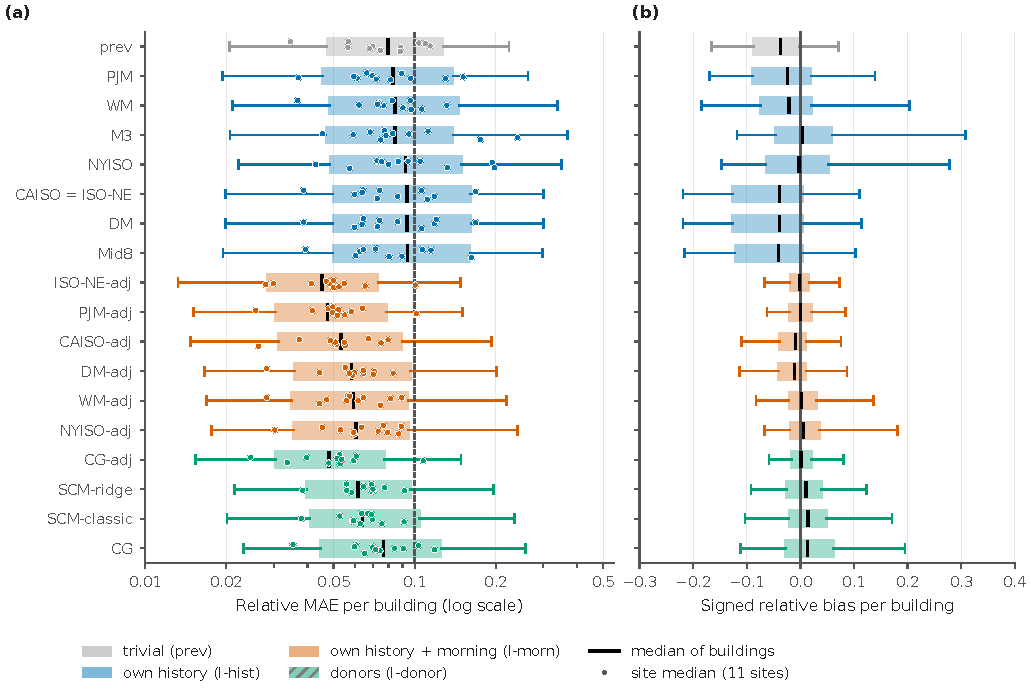
\includegraphics[width=\FigD]{figures/fig_03_accuracy.pdf}
\caption{Hot-day accuracy by method, grouped by information set ($n=9{,}550$ building-events at 11 sites). (a) relMAE: boxes show the building-level interquartile range, points the site medians; donor boxes are hatched. (b) Signed bias ($e=B-L$; negative means under-prediction). CAISO and ISO-NE unadjusted baselines coincide.}\label{fig:accuracy}
\end{figure}

%%FLOAT fig:h2h3
\begin{figure}[tp]
\centering
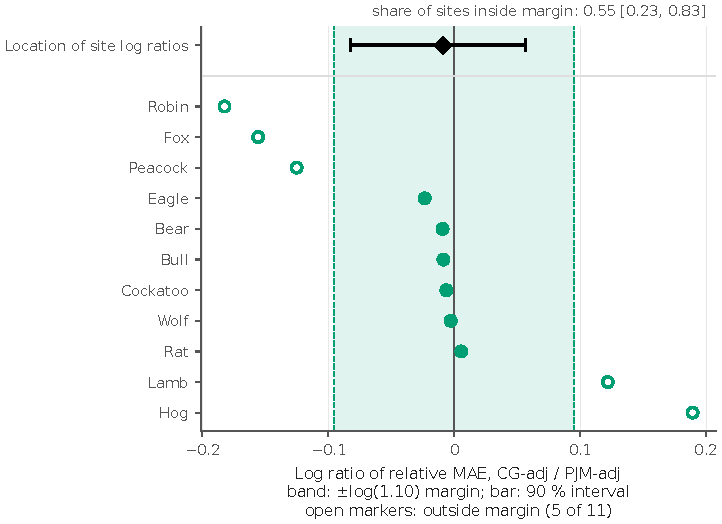
\includegraphics[width=0.78\linewidth]{figures/fig_05_h3_forest.pdf}
\caption{H3: site-level log ratios of relMAE, CG-adj over PJM-adj (11 sites), with the pre-set equivalence margin. The Hodges-Lehmann estimate (90\,\% interval) is the signed-rank location of the site values under the symmetry assumption; 5 of 11 sites lie outside the margin, so equivalence does not hold site by site. The H2 site values are in Supplement Fig.~\ref{figS:h2}.}\label{fig:h2h3}
\end{figure}

%%FLOAT fig:precool
\begin{figure}[tp]
\centering
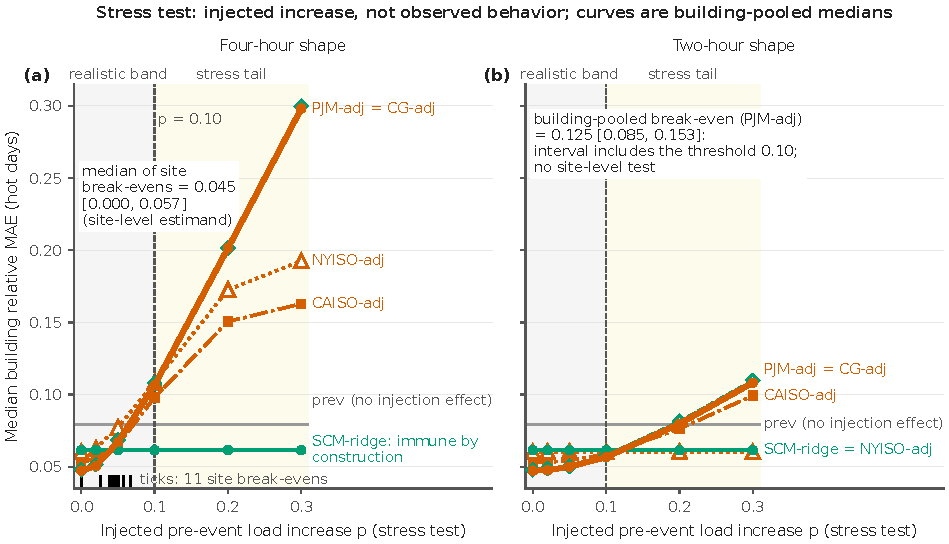
\includegraphics[width=\FigD]{figures/fig_06_precool.pdf}
\caption{Injected stress test: building-pooled median relMAE against the injected pre-event increase for the (a) four-hour and (b) two-hour shape ($n=9{,}550$ hot-day building-events at 11 sites). The plotted curves are building-pooled. The annotation in (a) is a separate estimand, the median of the 11 site break-even pre-event increases (4.5\,\%, order-statistic interval 0.0\,\% to 5.7\,\%, coverage at least 95\,\%), and the ticks mark the site values; 2 sites have a break-even of zero. In (b) the building-pooled interval (8.5\,\% to 15.3\,\%) includes the threshold of 0.10, and no site-level two-hour test was run. SCM-ridge is immune by construction to the specified four-hour injection. The four-hour shape covers all three PJM adjustment hours, so the break-even is a worst-case placement bound (Supplement Fig.~\ref{figS:placement}). Shaded: assumed realistic band.}\label{fig:precool}
\end{figure}

%%FLOAT fig:pstar
\begin{figure}[tp]
\centering
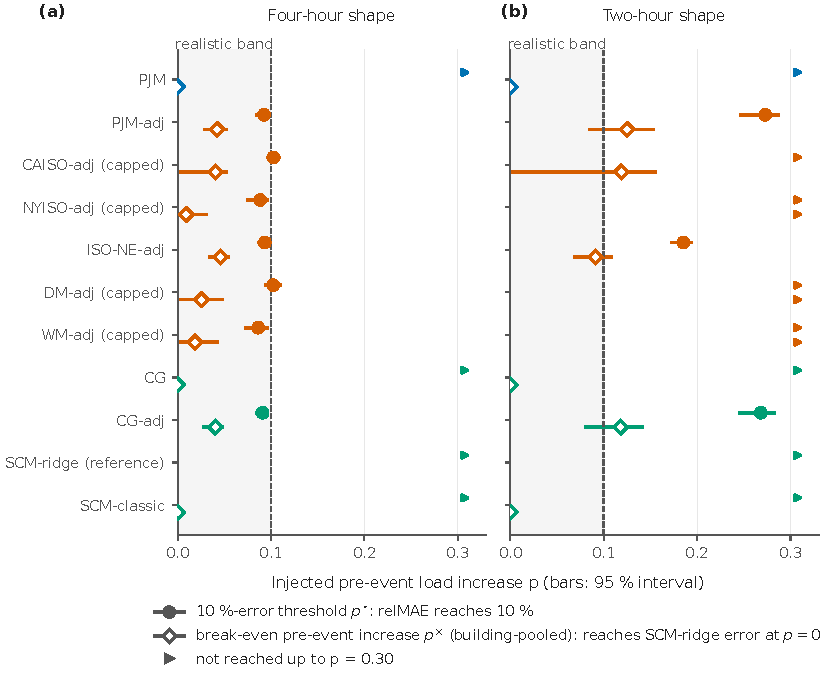
\includegraphics[width=\FigM]{figures/fig_07_pstar.pdf}
\caption{Stress test: building-pooled 10\,\%-error threshold $p^{\star}$ (relMAE reaches the curtailment value) and break-even pre-event increase $p^{\times}$ against SCM-ridge for each baseline, four-hour and two-hour shapes, ordered by information set, with 95\,\% intervals. Arrows mark values above the grid maximum; capped rules are marked. Shaded: assumed realistic band, an assumption and not derived from these data.}\label{fig:pstar}
\end{figure}

%%FLOAT fig:dispatch
\begin{figure}[tp]
\centering
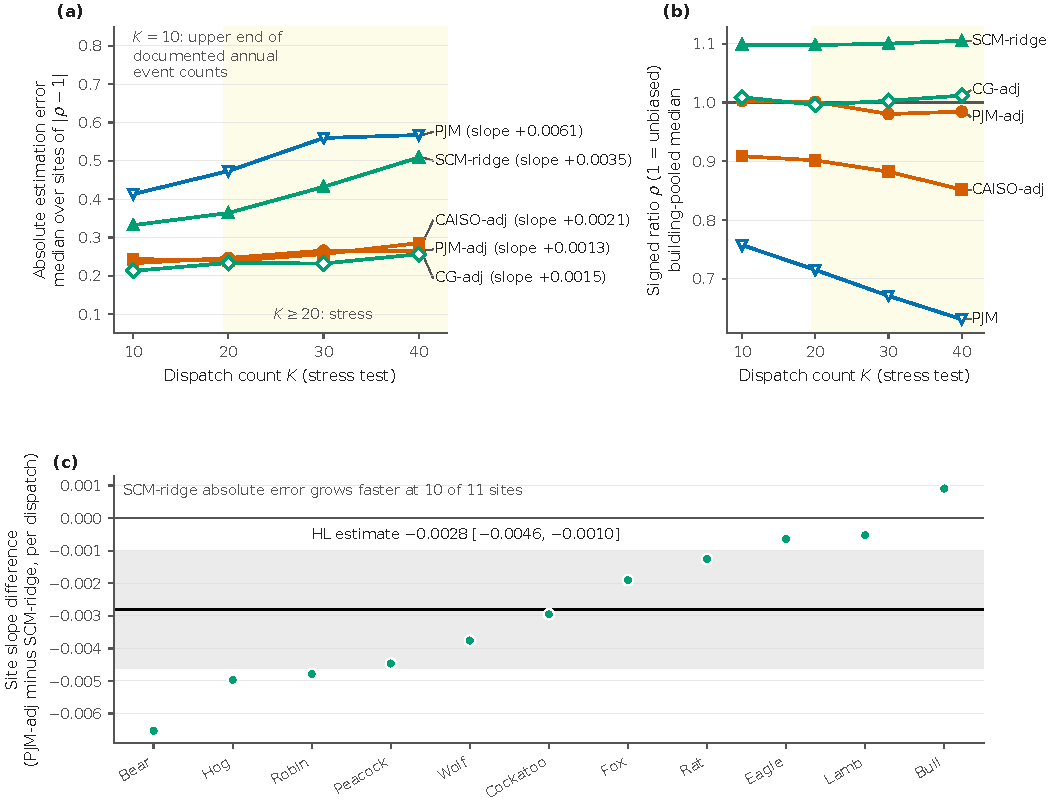
\includegraphics[width=\FigD]{figures/fig_08_dispatch.pdf}
\caption{Injected repeated-dispatch stress test by number of dispatched days $K$, confirmatory 14:00 to 18:00 window (11 sites). (a) Absolute estimation error (site median of $|\rho-1|$): PJM-adj stayed more accurate than SCM-ridge at each tested $K$, and both slopes are positive. (b) Signed ratio $\rho$. (c) Per-site slope differences, PJM-adj minus SCM-ridge, with the Hodges-Lehmann estimate $-$0.0028 (95\,\% interval $-$0.0046 to $-$0.0010); SCM-ridge's error grew faster at 10 of 11 sites. Values of $K$ above ten are stress levels. The pre-specified secondary 16:00 to 20:00 window is compared in Table~\ref{tab:h5windows}.}\label{fig:dispatch}
\end{figure}

%%FLOAT tab:h5windows
\begin{table}[tp]
\centering
\caption{H5, injected repeated-dispatch stress test: the level ordering and the slope contrast in the confirmatory 14:00 to 18:00 window and the pre-specified secondary 16:00 to 20:00 rerun (11 sites). PJM-adj has the lower site-median absolute error $|\rho-1|$ at 4 of 4 tested $K$ in the confirmatory window and 4 of 4 in the rerun. The slope contrast is confirmed at 14:00 to 18:00 (Holm-adjusted $p=0.0098$) and inconclusive at 16:00 to 20:00 (interval includes zero, unadjusted $p=0.365$). Values of $K$ above ten are stress levels. The exploratory cross-window contrast is in the table note.}\label{tab:h5windows}
\scriptsize
\begin{tabular}{lrr}
\toprule
 & 14:00-18:00 (confirmatory) & 16:00-20:00 (pre-specified secondary) \\
\midrule
Site-median $|\rho-1|$, $K = 10$, PJM-adj & 0.233 & 0.203 \\
Site-median $|\rho-1|$, $K = 10$, SCM-ridge & 0.332 & 0.342 \\
Site-median $|\rho-1|$, $K = 40$, PJM-adj & 0.265 & 0.258 \\
Site-median $|\rho-1|$, $K = 40$, SCM-ridge & 0.509 & 0.442 \\
$K$ (of 4) where PJM-adj is lower & 4 of 4 & 4 of 4 \\
Slope contrast, HL [95 \% CI] ($\times 10^{{-}3}$ per $K$) & $-$2.81 [$-$4.62, $-$1.02] & $-$0.75 [$-$3.39, $+$2.17] \\
$p$-value (exact signed-rank) & 0.0098 (Holm) & 0.365 (unadjusted) \\
Sites with SCM-ridge's error growing faster & 10 of 11 & 7 of 11 \\
\bottomrule
\end{tabular}
\par\smallskip{\footnotesize\raggedright PJM-adj, PJM rule with same-day adjustment; SCM-ridge, ridge synthetic control from other buildings; HL, Hodges-Lehmann estimate; CI, confidence interval; $K$, number of dispatched days. Site-median values are medians over the 11 sites of each site's median absolute error $|\rho-1|$. The slope contrast is the per-site slope of the site-median error over $K$ for PJM-adj minus SCM-ridge; negative means SCM-ridge's error grows faster. The 14:00-18:00 window is the confirmatory test (Holm-adjusted within the confirmatory family); 16:00-20:00 is a pre-specified secondary rerun with no adjustment. The windows are not pooled. Exploratory cross-window contrast (14:00-18:00 minus 16:00-20:00, per-site paired): HL $-$1.61 ($\times 10^{{-}3}$ per $K$), 95\,\% CI [$-$5.28, $+$0.26], unadjusted $p=0.10$.\par}

\end{table}

%%FLOAT fig:payment
\begin{figure}[tp]
\centering
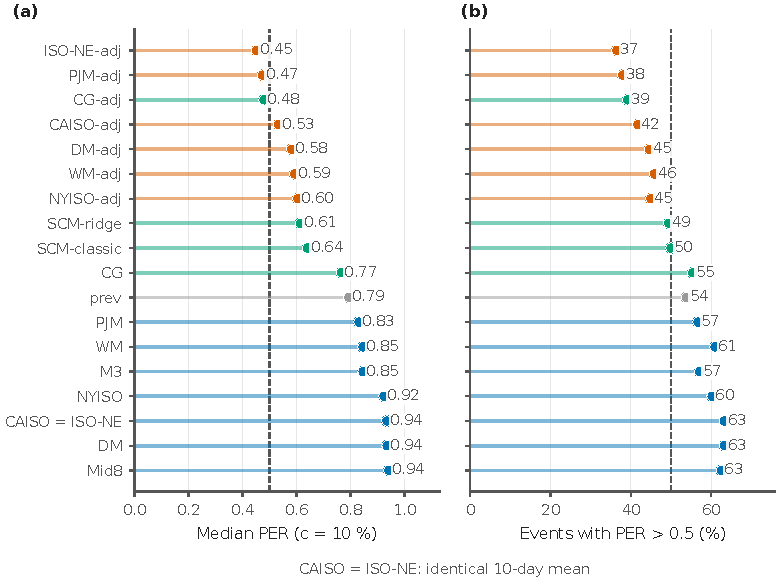
\includegraphics[width=\FigM]{figures/fig_10_payment.pdf}
\caption{Payment error ratio (PER), the hot-day error relative to the value of a ten percent curtailment, by method, sorted by median ($n=9{,}550$ hot-day building-events). The median PER is 0.47 for PJM-adj, 0.48 for CG-adj and 0.61 for SCM-ridge; the line marks one half.}\label{fig:payment}
\end{figure}

%%FLOAT tab:confirmatory
\begin{table}[tp]
\centering
\caption{Confirmatory tests H1 to H5 at 11 sites: estimand, estimate, interval, raw and Holm-adjusted $p$-values, decision and leave-one-site-out (LOSO) range. H3 is an equivalence test (TOST) and H4 an exact sign test; the others are exact signed-rank tests. LOSO is an influence analysis, not a replication; the exact $p$-values cannot fall below the enumeration floor for 11 sites.}\label{tab:confirmatory}
\scriptsize
\setlength{\tabcolsep}{2.5pt}
\begin{tabular}{l>{\raggedright\arraybackslash}p{4.3cm}rlrrll}
\toprule
Test & Estimand & Estimate & Interval & Raw p & Holm p & Decision & LOSO range \\
\midrule
H1 & $\Delta$ bias, PJM (hot day minus random weekday) & $-$0.0485 & [$-$0.0956, $-$0.0098] & 0.00146 & 0.00439 & supported & [$-$0.0541, $-$0.0421] \\
H2 & Log ratio relMAE, PJM-adj / PJM & $-$0.3976 & [$-$0.6253, $-$0.2232] & 0.00049 & 0.00244 & supported & [$-$0.4611, $-$0.3570] \\
H3 & Log ratio relMAE, CG-adj / PJM-adj (margin log 1.10) & $-$0.0089 & [$-$0.0824, 0.0564] & 0.01611 & 0.01611 & equivalent (TOST) & [$-$0.0163, $-$0.0062] \\
H4 & Median of the site break-even pre-event increases, PJM-adj vs SCM-ridge, four-hour stress test (order-statistic interval, coverage at least 95 \%; exact sign test) & 0.0448 & [0.0000, 0.0573] & 0.00049 & 0.00244 & supported & [0.0428, 0.0457] \\
H5 & Absolute-error growth per dispatch, PJM-adj minus SCM-ridge (negative: SCM-ridge grows faster) & $-$0.0028 & [$-$0.0046, $-$0.0010] & 0.00488 & 0.00977 & supported & [$-$0.0031, $-$0.0025] \\
\bottomrule
\end{tabular}
\par\smallskip{\footnotesize\raggedright Intervals are 95\,\% except for H3 (90\,\%); the H3 raw p is the TOST p-value. H4 is the median of the 11 site-level break-even pre-event increases; its LOSO range is on site medians. Building-pooled (secondary): break-even 0.0424, 95\,\% interval [0.0288, 0.0519]; this value pools buildings and is not the confirmatory statistic.\par}

\end{table}

